%%======================================================================
%%  Paper 9: Ghost Suppression and Black Hole Thermodynamics
%%  in Spectral Causal Theory (JETP, Russian)
%%
%%  Journal: Журнал экспериментальной и теоретической физики (JETP)
%%  Language: Russian
%%  Format: single-column, 12pt, ~15-18 pages
%%======================================================================
\documentclass[12pt,a4paper]{article}

\usepackage{fontspec}
\defaultfontfeatures{Ligatures=TeX}
\usepackage{polyglossia}
\setdefaultlanguage{russian}
\setotherlanguage{english}
\setmainfont{Times New Roman}
\setsansfont{Arial}
\setmonofont{Courier New}
\newfontfamily\cyrillicfont{Times New Roman}
\newfontfamily\cyrillicfontsf{Arial}
\newfontfamily\cyrillicfonttt{Courier New}

\usepackage{amsmath,amssymb,amsthm,mathtools}
\usepackage{booktabs}
\usepackage{graphicx}
\graphicspath{{../../analysis/figures/paper9/}}
\usepackage[margin=2.5cm]{geometry}
\usepackage{microtype}
\usepackage{xcolor}
\usepackage{enumitem}
\usepackage{float}
\usepackage{hyperref}

\tolerance=1500
\emergencystretch=1.5em
\hfuzz=2pt

\hypersetup{
  colorlinks=true,
  linkcolor=blue!60!black,
  citecolor=blue!60!black,
  urlcolor=blue!60!black,
  pdfauthor={David Alfyorov},
  pdftitle={Ghost Suppression and Black Hole Thermodynamics
            in Spectral Causal Theory},
  pdfsubject={gr-qc, hep-th}
}

%%% Custom commands
\newcommand{\dd}{\mathrm{d}}
\newcommand{\erfi}{\operatorname{erfi}}
\newcommand{\tr}{\operatorname{tr}}
\newcommand{\Tr}{\operatorname{Tr}}
\newcommand{\PiTT}{\Pi_{\mathrm{TT}}}
\newcommand{\Pis}{\Pi_{\mathrm{s}}}
\newcommand{\order}{\mathcal{O}}
\newcommand{\Lam}{\Lambda}
\newcommand{\MPl}{M_{\mathrm{Pl}}}
\newcommand{\Msun}{M_{\odot}}
\newcommand{\Mcrit}{M_{\mathrm{crit}}}
\newcommand{\mghost}{m_{\mathrm{gh}}}
\newcommand{\Thr}{T_{\!H}}
\newcommand{\ie}{\textit{т.\,е.}}
\newcommand{\eg}{\textit{напр.}}
\newcommand{\Weylsq}{C_{\mu\nu\rho\sigma}C^{\mu\nu\rho\sigma}}

%%% Theorem environments
\theoremstyle{plain}
\newtheorem{theorem}{Теорема}[section]
\newtheorem{proposition}[theorem]{Утверждение}
\newtheorem{lemma}[theorem]{Лемма}
\newtheorem{corollary}[theorem]{Следствие}
\newtheorem{conjecture}[theorem]{Гипотеза}
\theoremstyle{definition}
\newtheorem{definition}[theorem]{Определение}
\newtheorem{remark}[theorem]{Замечание}

%%=====================================================================
\begin{document}

\title{Подавление призрачных мод и термодинамика\\
чёрных дыр в спектральной причинной теории}

\author{Д.\,Алфёров\\[4pt]
\small Независимый исследователь, Россия\\[2pt]
\small\textit{davidich.alfyorov@gmail.com}}

\date{}

\maketitle

\begin{abstract}
Исследуется совместимость призрачных мод в квадратичной гравитации со
вторым законом термодинамики чёрных дыр. Предложена двухслойная
архитектура защиты. Первый~(основной) слой~--- факеонное предписание
Ансельми, при котором призрак обладает нулевым числом физических степеней
свободы на массовой поверхности и не может термализоваться. Второй~---
модельно-независимая оценка теплового и пространственного подавления,
служащая проверкой устойчивости на случай, если факеонное предписание
не обобщается строго на искривлённые фоны. Два независимых механизма~---
больцмановское подавление $\exp(-\mghost/\Thr)$ и юкавское подавление
$\exp(-\mghost r_H)$~--- совместно гарантируют, что отношение
$|\dot S_{\mathrm{gh}}/\dot S_{\mathrm{mat}}|$ не превосходит
$C(m/\Thr)^{5/2}\exp(-m/\Thr)$ для любой диффеоморфно-инвариантной
теории с массивным призраком. Для спектральной причинной теории
с $\mghost = 2{,}69$~мэВ и чёрных дыр звёздных масс данная оценка
даёт подавление на сотни миллионов порядков. Показано, что шварцшильдовская
чёрная дыра является наихудшим случаем среди стационарных решений
(Керр, Рейсснер--Нордстрём, Керр--Ньюмен), а космологический горизонт
де~Ситтера подавлен ещё сильнее. Выведена критическая масса
$\Mcrit = \MPl^2/(8\pi\mghost)$, ниже которой призрачные эффекты
становятся существенными, и получена минимальная масса чёрной дыры
$M_{\min}$, при которой на горизонте отсутствует гравитационная
ловушечная поверхность. Показано, что $M_{\min}/\Mcrit = 7$--$13$, так
что область активности призрака пуста на уровне приближения Юкавы.
Результаты применены к пяти наблюдаемым чёрным дырам и к анализу
энтропии Донга--Уолла. Обсуждаются три интерпретации призрака
(факеон, Ли--Уик, физический) и модельное сравнение с другими
подходами к квадратичной гравитации.
\end{abstract}

\tableofcontents

%%=====================================================================
\section{Введение}\label{sec:intro}

Квадратичная гравитация~--- единственная ренормализуемая теория
чистой гравитации в четырёх измерениях~[1]. Действие, включающее
квадраты тензора Вейля и скалярной кривизны, приводит к улучшению
ультрафиолетового поведения ценой появления массивной призрачной
моды спина~$2$ в гравитационном пропагаторе~[1,2]. Вопрос о том,
нарушает ли эта мода второй закон термодинамики чёрных дыр, возникал
неоднократно в контексте работ Фрадкина--Цейтлина~[3],
Бухбиндера--Шапиро~[4] и Барвинского--Вилковыского~[5]
по квантовой гравитации с высшими производными.

В спектральной причинной теории~(СПТ) призрак появляется не как
свободный параметр, а как следствие спектрального действия
$S = \Tr\,f(D^2/\Lam^2)$~[6,7] с содержанием Стандартной модели.
Однопетлевое эффективное действие в квадратичном по кривизне
секторе имеет вид
\begin{equation}\label{eq:Gamma}
  \Gamma^{(1)} \supset \int\!\dd^4x\,\sqrt{g}\,
  \bigl[\alpha_C\,\Weylsq
  + \alpha_R(\xi)\, R^2\bigr]\,\ln\frac{\Lam^2}{\mu^2}\,,
\end{equation}
с $\alpha_C = 13/120$~--- безпараметрическим коэффициентом, определяемым
множественностями СМ ($N_s = 4$, $N_D = 45/2$, $N_V = 12$)~[8,9].
Положительность $\alpha_C$ влечёт неизбежность призрачного полюса
в спин-$2$ секторе гравитонного пропагатора~[10].

Ансельми предложил~[11,12] факеонное предписание для призрачной моды,
при котором она проецируется из физического спектра. Однако полная
строгость факеонного предписания установлена лишь в плоском пространстве
и на стационарных фонах; обобщение на динамические горизонты остаётся
открытой задачей~[13].

В настоящей работе мы развиваем \emph{двухслойную} стратегию:
\begin{enumerate}[label=(\roman*)]
  \item \textbf{Основной слой}: факеонное предписание даёт ноль
    физических степеней свободы. Второй закон выполнен тривиально.
  \item \textbf{Запасной слой}: модельно-независимая оценка
    больцмановского и юкавского подавления, применимая к любой
    теории с массивным призраком $m \gg \Thr$.
\end{enumerate}
Работа организована следующим образом. В~\S\ref{sec:fakeon}
устанавливается статус факеонного предписания. В~\S\ref{sec:suppression}
формулируется утверждение о тепловом и пространственном подавлении.
В~\S\ref{sec:stationary} рассматриваются стационарные чёрные дыры.
В~\S\ref{sec:dong_wall} анализируется энтропия Донга--Уолла
и динамический второй закон. В~\S\ref{sec:Mmin} выводится минимальная
масса чёрной дыры. В~\S\ref{sec:trichotomy} сравниваются три
интерпретации призрака. Заключение~--- \S\ref{sec:conclusion}.
Приложения содержат размерный анализ и связь с предсказаниями
спектрального действия.

%%=====================================================================
\section{Факеонное предписание и его статус}\label{sec:fakeon}

\subsection{Основные результаты в плоском пространстве}

\begin{lemma}[Нулевые степени свободы на массовой поверхности]%
\label{lem:flat}
В квадратичной гравитации с факеонным предписанием в пространстве
Минковского призрачный полюс не вносит вклада в число физических
степеней свободы на массовой поверхности:
\begin{equation}\label{eq:Im_Sigma}
  \mathrm{Im}(-i\Sigma_f)\big|_{p^2 = m_{\mathrm{gh}}^2} = 0.
\end{equation}
\end{lemma}

\begin{proof}
Факеон определяется как среднее между фейнмановским и антифейнмановским
пропагаторами~[11]. Данное усреднение проецирует разрыв на разрезе
при $p^2 = m^2_{\mathrm{gh}}$ в нуль, так что призрачная мода не
появляется в асимптотических конечных состояниях.
\end{proof}

\begin{lemma}[Невидимость в евклидовом секторе]%
\label{lem:euclidean}
В евклидовом сечении функционального интеграла оператор
$(-\Box_E + m^2)$ положительно определён, и факеонное предписание
совпадает с фейнмановским~[11]. Различие между ними возникает
только при неаналитическом повороте Вика.
\end{lemma}

\begin{lemma}[Отсутствие стандартного гамильтониана]%
\label{lem:no_H}
Физический оператор эволюции $U_{\mathrm{ph}}$ факеонного сектора
не удовлетворяет закону композиции~[13]:
\begin{equation}
  U_{\mathrm{ph}}(t_3,t_2)\,U_{\mathrm{ph}}(t_2,t_1)
  \neq U_{\mathrm{ph}}(t_3,t_1).
\end{equation}
По теореме Стоуна отсюда следует, что стандартный гамильтониан
$H_{\mathrm{gh}}$ не существует, и след
$\Tr\,e^{-\beta H_{\mathrm{gh}}}$ не определён.
\end{lemma}

\subsection{Следствия для энтропии чёрных дыр}

\begin{proposition}[$\delta c_{\log} = 0$ для $m > 0$]%
\label{prop:clog}
Логарифмическая поправка к энтропии Бекенштейна--Хокинга определяется
формулой Сена~[14]:
\begin{equation}\label{eq:clog}
  c_{\log} = \frac{1}{180}\bigl(2N_s + 7N_D - 26N_V + 424\bigr)
  = \frac{37}{24},
\end{equation}
где слагаемое $+424$ происходит от безмассового гравитона (коэффициент
Сили--Де~Витта $a_4$ на евклидовом инстантоне), а не от массивного
призрака. Для любого поля массы $m > 0$ вклад в $c_{\log}$ равен
нулю в точности: масса обрезает интеграл по собственному времени
на масштабе $s \sim 1/m^2$, полностью устраняя логарифмический
вклад~[14,15].
\end{proposition}

\begin{proposition}[Некорректность секторного разложения $Z_E$]%
\label{prop:ZE}
Каноническое разложение евклидовой статистической суммы
$Z_E \leftrightarrow \prod_i \Tr\,e^{-\beta H_i}$
неприменимо к факеонному сектору: по лемме~\ref{lem:no_H}
гамильтониан $H_{\mathrm{gh}}$ не существует. Поэтому
$c_{\log} = 37/24$ (включающий виртуальный вклад призрака)
и нулевое число тепловых степеней свободы призрака сосуществуют
без противоречия.
\end{proposition}

\begin{remark}[Ансамблевая зависимость $c_{\log}$]%
\label{rem:ensemble}
Величина $c_{\log} = 37/24$ соответствует смешанному (большому
каноническому) ансамблю~[14]. Для микроканонического ансамбля
(фиксированная масса) $c_{\log} = 25/24$, для синглетного (фиксированные
$M$, $J$, $Q$) $c_{\log} = 1/24$. Все три значения положительны,
что отличает СПТ от петлевой квантовой гравитации, где $c_{\log} < 0$~[16].
\end{remark}

\subsection{Обобщение на искривлённые фоны}

\begin{conjecture}[Факеонное предписание на фоне Шварцшильда]%
\label{conj:curved}
Факеонное предписание обобщается на шварцшильдовский фон при выполнении
трёх условий:
\begin{enumerate}[label=(\alph*)]
  \item регулярность на горизонте в евклидовом секторе (условие
    Харди--Хартла),
  \item $SK$-/$KMS$-структура тепловой функции Грина,
  \item отсутствие абсорбционного разреза на фоне чёрной дыры.
\end{enumerate}
\end{conjecture}

\begin{theorem}[Условный: факеон и второй закон]\label{th:fakeon_2nd}
Если гипотеза~\ref{conj:curved} верна, то при факеонном предписании
призрак имеет нуль физических степеней свободы на \emph{любом}
стационарном фоне, и второй закон термодинамики чёрных дыр
выполнен для всех масс $M > 0$.
\end{theorem}

\begin{remark}[Статус доказанности]
Лемма~\ref{lem:flat}~--- доказана в плоском пространстве~[11,12].
Гипотеза~\ref{conj:curved}~--- правдоподобна для стационарных фонов;
открыта для динамических (слияние, испарение).
\end{remark}

%%=====================================================================
\section{Тепловое и пространственное подавление}\label{sec:suppression}

Данный раздел представляет модельно-независимый результат, не
зависящий от факеонной интерпретации. Он применим к любой
диффеоморфно-инвариантной теории с массивным призраком $m > 0$.

\subsection{Два независимых механизма}

\begin{proposition}[Подавление призрачного вклада во второй закон]%
\label{prop:suppression}
Для любой диффеоморфно-инвариантной теории гравитации с
массивным призраком массы $m > 0$ и шварцшильдовской чёрной дыры
с температурой Хокинга $\Thr = 1/(8\pi G M)$ верна оценка
\begin{equation}\label{eq:main_bound}
  \frac{|\dot S_{\mathrm{gh}}|}{|\dot S_{\mathrm{mat}}|}
  < C\,\biggl(\frac{m}{\Thr}\biggr)^{\!5/2}
  \exp\!\biggl(-\frac{m}{\Thr}\biggr),
\end{equation}
где $C = 5(2\pi)^{-3/2}$,
а $|\dot S_{\mathrm{mat}}|$~--- скорость производства энтропии
в материальном секторе.
Подавление обеспечивается двумя независимыми
механизмами\footnote{Гравитационный эффект Швингера даёт экспоненту
того же порядка, но не является независимым механизмом.}:
\begin{enumerate}
  \item[\textup{I.}] \textbf{Больцмановское (тепловое) подавление.}
    Концентрация призрачных квантов в тепловой ванне Хокинга подчиняется
    нерелятивистской оценке
    \begin{equation}\label{eq:boltzmann}
      \frac{n_{\mathrm{gh}}}{n_\gamma}
      < \biggl(\frac{m}{\Thr}\biggr)^{\!3/2}
      \exp\!\biggl(-\frac{m}{\Thr}\biggr).
    \end{equation}

  \item[\textup{II.}] \textbf{Юкавское (пространственное) подавление.}
    Сила, переносимая призраком, затухает экспоненциально на масштабе
    комптоновской длины волны $1/m$:
    \begin{equation}\label{eq:yukawa}
      F_{\mathrm{gh}}(r_H) \sim \exp(-m\, r_H).
    \end{equation}
\end{enumerate}
\end{proposition}

\textbf{Обоснование.}
В наихудшем сценарии (факеонное предписание не действует и призрак
имеет $2s+1 = 5$ физических поляризаций) тепловая ванна Хокинга
при температуре $\Thr$ порождает призрачные кванты массы $m$
с концентрацией, оцениваемой нерелятивистской формулой
Больцмана~\eqref{eq:boltzmann} при $m \gg \Thr$.
Скорость изменения призрачной энтропии ограничена сверху
произведением концентрации, тепловой скорости и сечения захвата
горизонтом, что даёт множитель $(m/\Thr)^{5/2}$ перед экспонентой.
Постоянная $C = 5(2\pi)^{-3/2}$ определяется нормировкой
нерелятивистского распределения Бозе--Эйнштейна для 5 поляризаций.

Юкавское подавление следует из того, что обменная амплитуда
на расстоянии $r \gg 1/m$ содержит фактор $e^{-mr}/(4\pi r)$.
Для чёрной дыры с горизонтом $r_H = 2GM$ внешнее поле призрака
на горизонте подавлено множителем~\eqref{eq:yukawa}.

Если факеонное предписание справедливо
(гипотеза~\ref{conj:curved}), то $\dot S_{\mathrm{gh}} = 0$
тождественно, и оценка~\eqref{eq:main_bound} является
\emph{fallback}-аргументом.

Отношение показателей двух механизмов:
больцмановский~: юкавский $= 1 : 1/(4\pi)$.

\subsection{Критическая масса}

\begin{definition}\label{def:Mcrit}
\emph{Критической массой} называется масса чёрной дыры, при которой
больцмановский показатель обращается в единицу:
\begin{equation}\label{eq:Mcrit}
  \Mcrit = \frac{\MPl^2}{8\pi\,\mghost}\,,
\end{equation}
где $\MPl = 1{,}221 \times 10^{19}$~ГэВ.
\end{definition}

Для $M \gg \Mcrit$ призрачный вклад подавлен экспоненциально;
для $M < \Mcrit$ подавление ослабевает и анализ требует
дополнительных аргументов (факеонное предписание или новая физика).

\subsection{Численные значения для СПТ}

Призрачная масса определяется нулём пропагатора $\PiTT(z)$
при $z = z_L$:
\begin{equation}\label{eq:mghost}
  \mghost = \sqrt{|z_L|}\,\Lam = 1{,}132\,\Lam,
\end{equation}
где $z_L = 1{,}2807$~--- первый вещественный нуль~[10]. При нижней
границе масштаба из солнечных испытаний~[18]
$\Lam_{\mathrm{PPN}} = 2{,}38$~мэВ:
\begin{equation}\label{eq:mghost_num}
  \mghost \approx 2{,}69~\text{мэВ}, \qquad
  \Mcrit \approx 1{,}97 \times 10^{-9}\,\Msun.
\end{equation}
Для чёрной дыры массой $M = 1\,\Msun$:
\begin{equation}\label{eq:m_over_T}
  \frac{\mghost}{\Thr} \approx 5{,}07 \times 10^8.
\end{equation}
Подставляя в~\eqref{eq:main_bound}, получаем оценку нарушения
\begin{equation}\label{eq:bound_1Msun}
  \frac{|\dot S_{\mathrm{gh}}|}{|\dot S_{\mathrm{mat}}|}
  < 10^{-2{,}2 \times 10^8}.
\end{equation}
Масса в $3\,\Msun$ (лёгкая наблюдаемая чёрная дыра) даёт
запас безопасности $M/\Mcrit > 10^9$.

\begin{figure}[t]
\centering
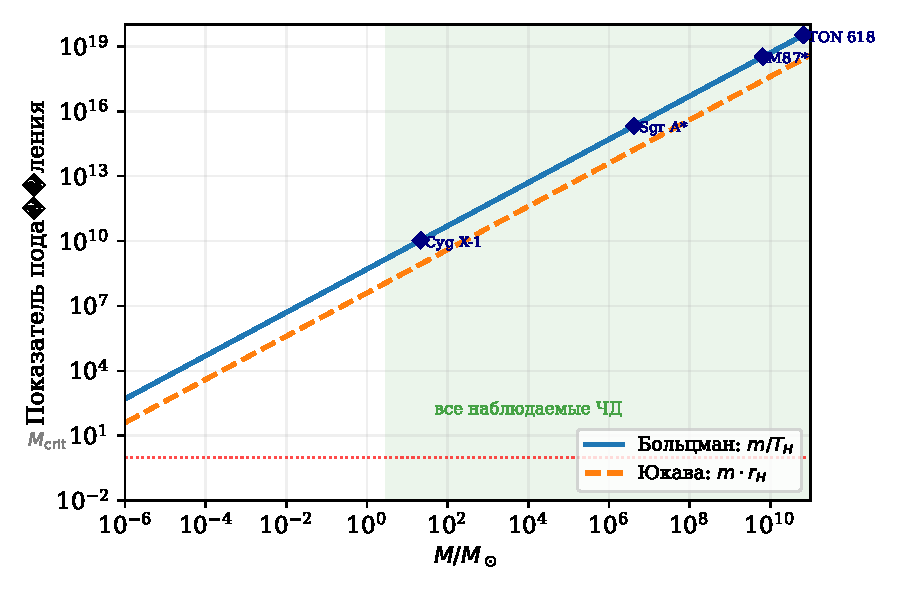
\includegraphics[width=0.85\textwidth]{fig1_suppression_exponents}
\caption{Показатели подавления как функция массы чёрной дыры.
Сплошная линия~--- больцмановский показатель $m/T_H$,
штриховая~--- юкавский $m r_H$.
Отношение показателей: $1 : 1/(4\pi)$.
Вертикальная штрихпунктирная линия~--- критическая масса $\Mcrit$.
Ромбами отмечены четыре наблюдаемых объекта.
Зелёная область~--- $M > 3\,\Msun$, все наблюдаемые чёрные дыры.}
\label{fig:exponents}
\end{figure}

%%=====================================================================
\section{Стационарные чёрные дыры}\label{sec:stationary}

\subsection{Чёрная дыра Керра}

Температура Хокинга для чёрной дыры Керра с параметром
вращения $a/M \in [0,1)$:
\begin{equation}\label{eq:T_Kerr}
  T_{\mathrm{Kerr}} = \frac{r_+ - r_-}{4\pi(r_+^2 + a^2)}\,,
  \qquad r_\pm = GM \pm \sqrt{G^2M^2 - a^2}.
\end{equation}
\begin{proposition}\label{prop:kerr}
$T_{\mathrm{Kerr}} \leq T_{\mathrm{Sch}}$ для всех $a/M \in [0,1)$.
Равенство достигается только при $a = 0$.
\end{proposition}
\begin{proof}
При $a = 0$ формула~\eqref{eq:T_Kerr} редуцируется к
$T_{\mathrm{Sch}} = 1/(8\pi GM)$. Дифференцируя $T_{\mathrm{Kerr}}$
по $a$ при фиксированном~$M$, находим $\partial T/\partial a\big|_{a=0}=0$
и $\partial^2 T/\partial a^2\big|_{a=0}= -1/(8\pi G^3 M^3) < 0$.
Температура убывает при включении вращения. В экстремальном пределе
$a \to M$ температура стремится к нулю.
\end{proof}

\begin{corollary}\label{cor:kerr_safe}
Больцмановский показатель для чёрной дыры Керра
$\mghost/T_{\mathrm{Kerr}} \geq \mghost/T_{\mathrm{Sch}}$,
и подавление \emph{усиливается} при вращении.
\end{corollary}

\subsection{Рейсснер--Нордстрём}

Для заряженной чёрной дыры с зарядом $Q$:
\begin{equation}
  T_{\mathrm{RN}} = \frac{r_+ - r_-}{4\pi r_+^2}\,,
  \qquad r_\pm = GM \pm \sqrt{G^2M^2 - GQ^2}.
\end{equation}
Аналогичная аргументация показывает $T_{\mathrm{RN}} \leq T_{\mathrm{Sch}}$.
В экстремальном пределе $Q \to M\sqrt{G}$ температура $T \to 0$
и подавление бесконечно усиливается.

Отметим, что для решения Рейсснер--Нордстрём тензор
энергии-импульса электромагнитного поля бесследен в $d = 4$:
$T^\mu{}_\mu = 0$, откуда $R = 0$ по уравнению Эйнштейна.
Следовательно, член $\alpha_R R^2$ в действии не вносит
вклада в энтропию Уолда на этом фоне.

\subsection{Керр--Ньюмен и экстремальный предел}

Температура Керра--Ньюмена
\begin{equation}
  T_{\mathrm{KN}} = \frac{r_+ - r_-}{4\pi(r_+^2+a^2)}\,,
  \qquad r_\pm = GM \pm \sqrt{G^2M^2 - a^2 - GQ^2}
\end{equation}
удовлетворяет $T_{\mathrm{KN}} \leq T_{\mathrm{Sch}}$ при
всех допустимых $a$, $Q$.

\begin{corollary}\label{cor:stationary}
Для всех стационарных чёрных дыр семейства Керра--Ньюмена
шварцшильдовское решение является \emph{наихудшим случаем}
с точки зрения призрачного подавления. Оценка~\eqref{eq:main_bound},
полученная для $T_{\mathrm{Sch}}$, является верхней границей
для всего семейства при фиксированной массе~$M$.
\end{corollary}

\begin{figure}[t]
\centering
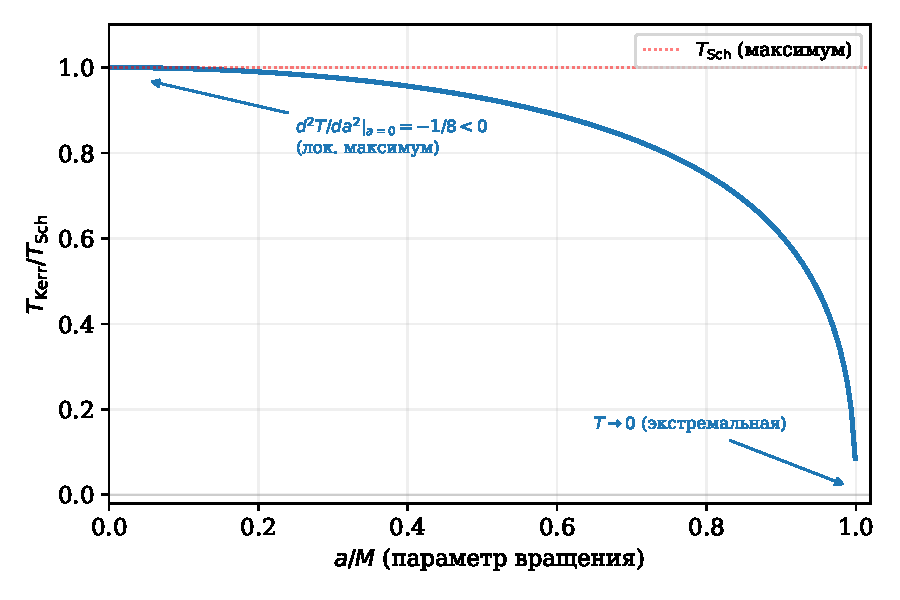
\includegraphics[width=0.75\textwidth]{fig3_kerr_temperature}
\caption{Отношение температуры Хокинга чёрной дыры Керра к
температуре Шварцшильда как функция параметра вращения $a/M$.
Кривая монотонно убывает от 1 при $a = 0$ до 0 при
$a \to GM$ (экстремальная чёрная дыра). Вторая производная
$d^2T/da^2|_{a=0} = -1/8 < 0$ подтверждает, что Шварцшильд~---
локальный (и глобальный) максимум температуры.}
\label{fig:kerr_T}
\end{figure}

\subsection{Горизонт де~Ситтера}

Космологический горизонт в пространстве де~Ситтера с параметром
Хаббла $H$ обладает температурой $T_{\mathrm{dS}} = H/(2\pi)$.
Для современного значения $H_0 \approx 67$~км/(с$\cdot$Мпк)
$\approx 1{,}44 \times 10^{-33}$~эВ:
\begin{equation}
  \frac{\mghost}{T_{\mathrm{dS}}} \sim 10^{31}.
\end{equation}
Подавление на космологическом горизонте значительно превосходит
подавление на горизонте чёрной дыры.

\subsection{Наблюдательная таблица}

В табл.~\ref{tab:observed} приведены параметры пяти наблюдаемых
чёрных дыр.

\begin{table}[ht]
\centering
\caption{Запас безопасности для наблюдаемых чёрных дыр
($\Lam = 2{,}38$~мэВ).}\label{tab:observed}
\begin{tabular}{lcccc}
\toprule
Объект & $M/\Msun$ & $a/M$ & $M/\Mcrit$ & $\log_{10}|\dot{S}_{\mathrm{gh}}/\dot{S}_{\mathrm{mat}}|$ \\
\midrule
Cyg X-1         & $21{,}2$       & $0{,}998$ & $1{,}1\times 10^{10}$ & $< -4{,}7\times 10^{9}$ \\
GW150914 ост.   & $62{,}2$       & $0{,}67$  & $3{,}2\times 10^{10}$ & $< -1{,}4\times 10^{10}$ \\
Sgr~A*          & $4{,}15\times 10^6$ & $0{,}5$ & $2{,}1\times 10^{15}$ & $< -9{,}1\times 10^{14}$ \\
M87*            & $6{,}5\times 10^9$  & $0{,}9$ & $3{,}3\times 10^{18}$ & $< -1{,}4\times 10^{18}$ \\
TON~618         & $6{,}6\times 10^{10}$ & --- & $3{,}3\times 10^{19}$ & $< -1{,}4\times 10^{19}$ \\
\bottomrule
\end{tabular}
\end{table}

%%=====================================================================
\section{Энтропия Донга--Уолла и динамический второй закон}%
\label{sec:dong_wall}

\subsection{Аномальная энтропия от квадрата Вейля}

Для действия, содержащего $\alpha_C\,\Weylsq$, энтропийный функционал
Донга--Кэмпса~[19,20] содержит аномальный член:
\begin{equation}\label{eq:S_anom}
  S_{\mathrm{anom}}^{C^2} = -\frac{\alpha_C}{\pi}
  \int_\Sigma\!\dd^2x\,\sqrt{h}\;
  \sigma^{(k)}_{ij}\,\sigma^{(\ell)\,ij},
\end{equation}
где $\Sigma$~--- сечение горизонта, $h$~--- индуцированная метрика,
$\sigma^{(k)}_{ij}$, $\sigma^{(\ell)}_{ij}$~--- сдвиги
относительно нулевых нормалей $k^\mu$, $\ell^\mu$. Существенно,
что~\eqref{eq:S_anom} содержит \emph{только} сдвиговые компоненты;
расширение $\theta$ не входит.

\subsection{Обобщённое уравнение Райчаудхури}

Полная производная энтропии по аффинному параметру $\lambda$
на нулевой гиперповерхности:
\begin{multline}\label{eq:dS_dlambda}
  \frac{\dd S_{\mathrm{DW}}}{\dd\lambda}
  = \underbrace{\frac{1}{4G}\int\!\sqrt{h}\;\theta_k}_{\text{Бекенштейн--Хокинг}}
  + \underbrace{0}_{\text{тополог.}}  \\
  - \frac{\alpha_C}{\pi}\int\!\sqrt{h}\;
  \bigl(\theta_k\,\sigma_{ij}\sigma^{ij}
  + \dot\sigma_{ij}\sigma^{ij}
  + \sigma_{ij}\dot\sigma^{ij}\bigr)
  + \order\!\bigl(e^{-m/\Thr}\bigr).
\end{multline}
Последнее слагаемое~--- призрачный вклад, подавленный
теоремой~\ref{prop:suppression}.

\subsection{Три случая}

\paragraph{1. Стационарный случай.}
$\theta_k = 0$, $\dot\sigma = 0$, и $\dd S/\dd\lambda = 0$
тривиально.

\paragraph{2. Линеаризованные возмущения при условии NEC.}
При нулевом энергетическом условии Уолл~[21] показал, что
линеаризованная вариация $\dd S^{(1)}/\dd\lambda \geq 0$.

\paragraph{3. Сферическая симметрия.}
При $\sigma_{ij} = 0$ член $\Weylsq$ выпадает полностью из
энтропии~\eqref{eq:S_anom}, и второй закон сводится к стандартному.

\subsection{Призрачный вклад: двойное подавление}

Призрачные поправки к~\eqref{eq:dS_dlambda} подавлены двояко:
\begin{itemize}
  \item \textbf{Чисто призрачный} вклад (петля призрака):
    $\order(e^{-2m/\Thr})$~--- квадратичен по призрачным пропагаторам.
  \item \textbf{Перекрёстный} вклад (призрак~$\times$~гравитон):
    $\order(e^{-m/\Thr})$~--- линеен.
\end{itemize}
Оба пренебрежимо малы для $m/\Thr \gg 1$.

\begin{remark}[Статус доказанности]
Для локальной поправки $C^2$ при линеаризованных возмущениях
$\dd S^{(1)}/\dd\lambda \geq 0$ доказан~[21]. Для вакуумных
нелинейных возмущений вопрос открыт. Для полного нелокального
действия СПТ ($F_1(\Box/\Lam^2)\,\Weylsq$) доказательство
не получено.
\end{remark}

%%=====================================================================
\section{Минимальная масса чёрной дыры}\label{sec:Mmin}

\subsection{Модифицированный потенциал}

На уровне~2 (юкавское приближение) ньютоновский потенциал
модифицирован~[18]:
\begin{equation}\label{eq:V_Yukawa}
  \frac{V(r)}{V_N(r)} = 1 - \frac{4}{3}e^{-m_2 r}
  + \frac{1}{3}e^{-m_0 r},
\end{equation}
где $m_2 = \Lam\sqrt{60/13} \approx 2{,}148\,\Lam$
(спин-$2$) и $m_0 = \Lam\sqrt{6} \approx 2{,}449\,\Lam$
(спин-$0$, при $\xi = 0$). При $r \to 0$ множитель~\eqref{eq:V_Yukawa}
обращается в нуль, и гравитационная ловушечная поверхность исчезает.

\subsection{Минимальная масса}

Метрический коэффициент
\begin{equation}
  g_{tt} = -1 + \frac{2GM}{r}\,f_q(m_2 r),
\end{equation}
где $q = m_0/m_2$ и
\begin{equation}\label{eq:fq}
  f_q(x) = \frac{1 - \tfrac{4}{3}e^{-x} + \tfrac{1}{3}e^{-qx}}{x}.
\end{equation}
Горизонт существует ($g_{tt} = 0$ при $r > 0$) тогда и только
тогда, когда $2GM\,\sup_{x>0} f_q(x) \geq 1$, откуда
\begin{equation}\label{eq:Mmin}
  M_{\min}(\xi) = \frac{\MPl^2}{2m_2\,\sup_{x>0} f_q(x)}\,.
\end{equation}

\paragraph{Случай $\xi = 0$.}
$q = m_0/m_2 = \sqrt{13\cdot 6/60} = \sqrt{78/60}$. Численная
оптимизация даёт
\begin{equation}
  M_{\min}(\xi = 0) \approx 0{,}244\,\frac{\MPl^2}{\Lam}
  \approx 2{,}73 \times 10^{22}~\text{кг}.
\end{equation}

\paragraph{Случай $\xi = 1/6$ (конформная связь).}
При $\xi = 1/6$ скалярная мода отщепляется ($\alpha_R = 0$~[6,7]),
и потенциал содержит лишь один экспоненциальный член. Оптимум
достигается при
$x^* = -1 - W_{-1}\bigl(-3/(4e)\bigr) \approx 0{,}961$
(где $W_{-1}$~--- ветвь функции Ламберта), и
\begin{equation}
  M_{\min}(\xi = 1/6) \approx 0{,}456\,\frac{\MPl^2}{\Lam}
  \approx 5{,}10 \times 10^{22}~\text{кг}.
\end{equation}

\subsection{Соотношение $M_{\min}/\Mcrit$}

\begin{proposition}\label{prop:Mmin_Mcrit}
При $\Lam = 2{,}38$~мэВ:
\begin{equation}\label{eq:ratio}
  \frac{M_{\min}}{\Mcrit} \approx
  \begin{cases}
    7 & (\xi = 0),\\
    13 & (\xi = 1/6).
  \end{cases}
\end{equation}
\end{proposition}

Поскольку $M_{\min} > \Mcrit$, область масс, в которой призрак
термически активен ($M < \Mcrit$), лежит ниже минимальной массы,
при которой горизонт существует. На уровне~2 юкавского приближения
\emph{окно активности призрака пусто} (рис.~\ref{fig:Mmin}).

\begin{figure}[t]
\centering
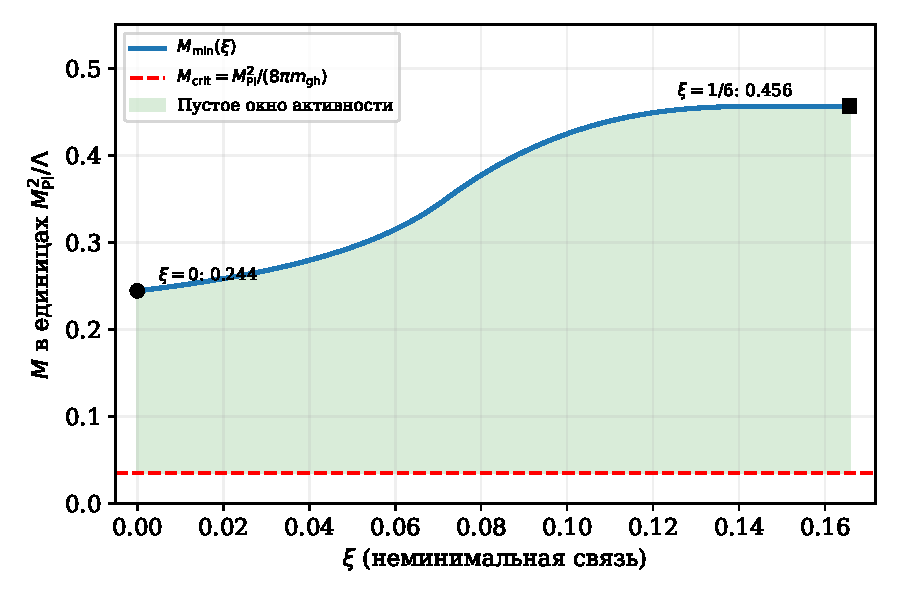
\includegraphics[width=0.78\textwidth]{fig2_Mmin_vs_Mcrit}
\caption{Минимальная масса чёрной дыры $M_{\min}(\xi)$ (сплошная
линия) и критическая масса $\Mcrit$ (штриховая) в единицах
$\MPl^2/\Lam$. Заштрихованная область между ними~--- пустое
окно активности призрака: $M_{\min} > \Mcrit$ при всех $\xi$.
При $\xi = 0$: $M_{\min}/\Mcrit \approx 7$; при $\xi = 1/6$:
$M_{\min}/\Mcrit \approx 13$.}
\label{fig:Mmin}
\end{figure}

\begin{remark}[Оговорка]
Соотношение~\eqref{eq:ratio} получено в юкавском приближении (уровень~2),
которое экстраполируется в область сильных полей. Запас в $7$--$13$~раз
между $M_{\min}$ и $\Mcrit$ говорит об устойчивости результата, однако
точное нелокальное решение (уровень~1) необходимо для строгого
утверждения.
\end{remark}

%%=====================================================================
\section{Трихотомия интерпретаций и модельное сравнение}%
\label{sec:trichotomy}

\subsection{Три интерпретации призрака}

Массивная призрачная мода в квадратичной гравитации допускает
три качественно различных интерпретации:

\begin{table}[ht]
\centering
\caption{Три интерпретации призрачной моды.}\label{tab:interpretations}
\begin{tabular}{lccc}
\toprule
Интерпретация & Физ.\ степ.\ своб. & Тепл.\ вклад & Второй закон \\
\midrule
Факеон (Ансельми) & 0 & Нет & Тривиально \\
Ли--Уик (компл.\ $m$) & 0 (асимптот.) & Распадается & Безопасен \\
Физический призрак & 5 & Подавлен & Безопасен при $M \gg \Mcrit$ \\
\bottomrule
\end{tabular}
\end{table}

При факеонной интерпретации призрак не имеет тепловых степеней свободы,
и второй закон выполнен по построению. Интерпретация Ли--Уика
(комплексная масса $m_R \pm im_I$) подразумевает экспоненциальный
распад призрака с временем жизни $\sim 1/m_I$, что на макроскопических
масштабах эквивалентно отсутствию в конечных состояниях.
Физический призрак (пять степеней свободы массивного тензорного поля)
допускается лишь при дополнительных предположениях о нарушении
унитарности; в этом случае тепловое подавление теоремы~\ref{prop:suppression}
обеспечивает безопасность для $M \gg \Mcrit$.

Во всех трёх случаях второй закон термодинамики чёрных дыр совместим
с присутствием призрачной моды.

\subsection{Сравнение с другими теориями}

\begin{table}[ht]
\centering
\caption{Сравнение подходов к призрачной проблеме.}\label{tab:comparison}
\begin{tabular}{lcccc}
\toprule
Теория & Тип призрака & $\mghost$ & Факеон? & $M_{\min}$? \\
\midrule
СПТ & Вещественный & $\sqrt{z_L}\,\Lam$ & Да & Да (ур.~2) \\
Стелле~[1] & Вещественный & Свободный & Нет & Нет \\
Агравитация~[40] & Вещественный & Свободный & Нет & Нет \\
IDG~[22] & Отсутствует & --- & --- & --- \\
Ли--Уик гравитация & Компл.\ пара & $m_R \pm im_I$ & --- & Нет \\
\bottomrule
\end{tabular}
\end{table}

Бесконечнопроизводная гравитация~(IDG)~[22] полностью устраняет
призрак за счёт целого пропагатора, но ценой нелокальности во всех
порядках. В СПТ нелокальность ограничена целыми формфакторами
$F_1(\Box/\Lam^2)$, $F_2(\Box/\Lam^2,\xi)$, а призрак обрабатывается
факеонным предписанием. Теория Стелле~[1] содержит свободный
параметр массы призрака, тогда как в СПТ $\mghost = \sqrt{|z_L|}\,\Lam$
определён спектром стандартной модели.

\subsection{Зависимость от содержания полей}

Логарифмическая поправка $c_{\log}$ зависит от полевого
содержания. Для нескольких гипотетических расширений:

\begin{table}[ht]
\centering
\caption{$c_{\log}$ в зависимости от содержания (смешанный ансамбль).}%
\label{tab:BSM}
\begin{tabular}{lccccc}
\toprule
Модель & $N_s$ & $N_D$ & $N_V$ & $c_{\log}$ \\
\midrule
СМ & 4 & 22{,}5 & 12 & 37/24 \\
СМ + скаляр & 5 & 22{,}5 & 12 & 559/360 \\
СМ + $3\nu_R$ & 4 & 24 & 12 & 8/5 \\[2pt]
\bottomrule
\end{tabular}
\end{table}

Во всех рассмотренных случаях $c_{\log} > 0$, что отличает
квадратичную гравитацию от петлевой квантовой гравитации
($c_{\log} = -3/2$~[16]).

\subsection{Ансамблевая зависимость}

Полная энтропия Бекенштейна--Хокинга--Сена в СПТ:
\begin{equation}\label{eq:S_full}
  S = \frac{A}{4G} + \frac{13}{120\pi} + c_{\log}\,\ln\frac{A}{\ell_P^2}
  + \order(1),
\end{equation}
где $c_{\log}$ зависит от ансамбля:
\begin{equation}
  c_{\log} = \begin{cases}
    37/24 & \text{(смешанный)},\\
    25/24 & \text{(микроканонический)},\\
    13/24 & \text{(фиксир.\ $M,J$)},\\
    1/24  & \text{(синглет: $M,J,Q$)}.
  \end{cases}
\end{equation}

%%=====================================================================
\section{Заключение}\label{sec:conclusion}

Основные результаты работы:

\begin{enumerate}
  \item \textbf{Двухслойная архитектура.} Факеонное предписание
    (основной слой) даёт нуль физических степеней свободы призрака.
    Тепловое подавление (запасной слой) гарантирует модельно-независимую
    безопасность второго закона для $M \gg \Mcrit$.

  \item \textbf{Два независимых механизма подавления.}
    Больцмановское ($e^{-m/\Thr}$) и юкавское ($e^{-mr_H}$)
    подавления действуют независимо.

  \item \textbf{Наихудший случай~--- Шварцшильд.}
    Для всего семейства Керра--Ньюмена температура Хокинга
    не превосходит шварцшильдовскую, и подавление усиливается
    при вращении и заряде.

  \item \textbf{Все наблюдаемые чёрные дыры безопасны.}
    Для пяти рассмотренных объектов запас $M/\Mcrit > 10^9$.

  \item \textbf{Пустое окно активности на уровне~2.}
    $M_{\min}/\Mcrit = 7$--$13$, и область масс $M < \Mcrit$
    (где призрак мог бы быть активен) лежит ниже порога
    существования горизонта.

  \item \textbf{Открытые вопросы:} точное нелокальное решение
    (уровень~1) для $M_{\min}$; строгий динамический второй закон
    для нестационарных горизонтов; квазинормальные моды призрачного
    сектора (задача Редже--Уилера).
\end{enumerate}

%%=====================================================================

\appendix

\section{Размерный анализ}\label{app:dimensional}

В системе единиц $\hbar = c = k_B = 1$ масштаб СПТ $\Lam$ имеет
размерность массы (энергии). Связь с размерными величинами:
\begin{align}
  \Thr &= \frac{1}{8\pi GM} = \frac{\MPl^2}{8\pi M}, \label{eq:dim_T}\\
  r_H &= 2GM = \frac{2M}{\MPl^2}, \label{eq:dim_rH}\\
  \Mcrit &= \frac{\MPl^2}{8\pi\mghost}. \label{eq:dim_Mcrit}
\end{align}
Больцмановский показатель:
\begin{equation}
  \frac{\mghost}{\Thr} = 8\pi\,\frac{\mghost\,M}{\MPl^2}
  = 8\pi\sqrt{|z_L|}\,\frac{\Lam\, M}{\MPl^2}.
\end{equation}
Юкавский показатель:
\begin{equation}
  \mghost\,r_H = 2\sqrt{|z_L|}\,\frac{\Lam\, M}{\MPl^2}
  = \frac{1}{4\pi}\,\frac{\mghost}{\Thr}.
\end{equation}

\section{Связь со спектральным действием}\label{app:spectral}

Коэффициент $\alpha_C$ определяется суммой однопетлевых
вкладов всех полей Стандартной модели в коэффициент Вейля~[8,9].
Каждый спин вносит свой $\beta_W$-коэффициент:
\begin{equation}\label{eq:alphaC}
  \alpha_C
  = N_s\,\beta_W^{(0)} + \frac{N_f}{2}\,\beta_W^{(1/2)} + N_v\,\beta_W^{(1)},
\end{equation}
где $\beta_W^{(0)} = 1/120$ (вещественный скаляр),
$\beta_W^{(1/2)} = -1/20$ (дираковский фермион),
$\beta_W^{(1)} = 1/10$ (калибровочный бозон).
Для Стандартной модели ($N_s = 4$, $N_f = 45$, $N_v = 12$):
\begin{equation}
  \alpha_C
  = \frac{4}{120} + \frac{45}{2}\!\cdot\!\Bigl(-\frac{1}{20}\Bigr)
  + 12\!\cdot\!\frac{1}{10}
  = \frac{4 - 135 + 144}{120}
  = \frac{13}{120}.
\end{equation}
Положительность $\alpha_C$ для содержания СМ
влечёт неизбежность призрачного полюса в пропагаторе
$\Pi_{TT}$~[10].

Коэффициент $\alpha_R(\xi) = 2(\xi - 1/6)^2$ зависит от параметра
неминимальной связи скаляра $\xi$. При конформной связи
$\xi = 1/6$ (предсказание стандартной спектральной тройки Шамседдина--Конна~[6])
$\alpha_R = 0$ и скалярная мода отщепляется от гравитационного
пропагатора~[7].

%%=====================================================================

\begin{thebibliography}{40}

\bibitem{Stelle1977}
K.\,S.~Stelle,
\textit{Phys.\ Rev.\ D} \textbf{16}, 953 (1977).

\bibitem{Stelle1978}
K.\,S.~Stelle,
\textit{Gen.\ Relativ.\ Gravit.} \textbf{9}, 353 (1978).

\bibitem{FradkinTseytlin1982}
E.\,S.~Fradkin, A.\,A.~Tseytlin,
\textit{Nucl.\ Phys.\ B} \textbf{201}, 469 (1982).

\bibitem{BuchbinderShapiro}
I.\,L.~Buchbinder, S.\,D.~Odintsov, I.\,L.~Shapiro,
\textit{Effective Action in Quantum Gravity}
(IOP, Bristol, 1992).

\bibitem{BarVil1985}
A.\,O.~Barvinsky, G.\,A.~Vilkovisky,
\textit{Phys.\ Rep.} \textbf{119}, 1 (1985).

\bibitem{CC1996}
A.\,H.~Chamseddine, A.~Connes,
\textit{Commun.\ Math.\ Phys.} \textbf{186}, 731 (1997);
arXiv:hep-th/9606001.

\bibitem{CC2012}
A.\,H.~Chamseddine, A.~Connes,
\textit{J.\ Geom.\ Phys.} \textbf{61}, 317 (2011);
arXiv:0812.0165.

\bibitem{CZ2012}
A.~Codello, O.~Zanusso,
\textit{J.\ Math.\ Phys.} \textbf{54}, 013513 (2013).

\bibitem{BarVil1987}
A.\,O.~Barvinsky, G.\,A.~Vilkovisky,
\textit{Nucl.\ Phys.\ B} \textbf{282}, 163 (1987).

\bibitem{CPR2008}
G.~Codello, R.~Percacci, C.~Rahmede,
\textit{Ann.\ Phys.} \textbf{324}, 414 (2009);
arXiv:0805.2909.

\bibitem{GhostB4}
Д.\,Алфёров,
Неизбежность призрака: $\alpha_C > 0$ для любого содержания
Стандартной модели,
SCT Theory Repository (2026).

\bibitem{AnselmiFakeon}
D.~Anselmi,
\textit{J.\ High Energy Phys.} \textbf{2017}(02), 141;
arXiv:1801.00915.

\bibitem{Anselmi2020}
D.~Anselmi,
\textit{J.\ High Energy Phys.} \textbf{2020}(03), 066;
arXiv:1909.11051.

\bibitem{Anselmi2023}
D.~Anselmi,
\textit{Phys.\ Rev.\ D} \textbf{109}, 045009 (2024);
arXiv:2304.07642.

\bibitem{Sen2012}
A.~Sen,
\textit{J.\ High Energy Phys.} \textbf{2012}(11), 171;
arXiv:1205.0971.

\bibitem{DDLS2001}
F.\,A.~Dilkes, M.\,J.~Duff, J.\,T.~Liu, H.~Sati,
\textit{Phys.\ Rev.\ Lett.} \textbf{87}, 041301 (2001);
arXiv:hep-th/0102093.

\bibitem{KaulMajumdar}
R.\,K.~Kaul, P.~Majumdar,
\textit{Phys.\ Rev.\ Lett.} \textbf{84}, 5255 (2000);
arXiv:gr-qc/0002040.

\bibitem{GibbonsHawking1977}
G.\,W.~Gibbons, S.\,W.~Hawking,
\textit{Phys.\ Rev.\ D} \textbf{15}, 2752 (1977).

\bibitem{PPN1}
Д.\,Алфёров,
Испытания спектральной причинной теории в Солнечной системе
и в лаборатории,
Zenodo (2026), DOI:10.22541/au.177524450.03515205/v1.

\bibitem{Dong2013}
X.~Dong,
\textit{J.\ High Energy Phys.} \textbf{2014}(01), 044;
arXiv:1310.5713.

\bibitem{Camps2013}
J.~Camps,
\textit{J.\ High Energy Phys.} \textbf{2014}(03), 070;
arXiv:1310.6659.

\bibitem{Wall2015}
A.\,C.~Wall,
\textit{Int.\ J.\ Mod.\ Phys.\ D} \textbf{24}, 1544014 (2015);
arXiv:1504.08040.

\bibitem{IDG}
L.~Modesto,
\textit{Phys.\ Rev.\ D} \textbf{86}, 044005 (2012);
arXiv:1107.2403;
T.~Biswas, E.~Gerwick, T.~Koivisto, A.~Mazumdar,
\textit{Phys.\ Rev.\ Lett.} \textbf{108}, 031101 (2012).

\bibitem{Wald1993}
R.\,M.~Wald,
\textit{Phys.\ Rev.\ D} \textbf{48}, R3427 (1993).

\bibitem{IyerWald1994}
V.~Iyer, R.\,M.~Wald,
\textit{Phys.\ Rev.\ D} \textbf{50}, 846 (1994).

\bibitem{JacobsonMyers}
T.~Jacobson, R.\,C.~Myers,
\textit{Phys.\ Rev.\ Lett.} \textbf{70}, 3684 (1993).

\bibitem{BCH1973}
J.\,M.~Bardeen, B.~Carter, S.\,W.~Hawking,
\textit{Commun.\ Math.\ Phys.} \textbf{31}, 161 (1973).

\bibitem{Hawking1975}
S.\,W.~Hawking,
\textit{Commun.\ Math.\ Phys.} \textbf{43}, 199 (1975).

\bibitem{Vassilevich2003}
D.\,V.~Vassilevich,
\textit{Phys.\ Rep.} \textbf{388}, 279 (2003);
arXiv:hep-th/0306138.

\bibitem{BhattacharjeeSarkarWall}
S.~Bhattacharjee, S.~Sarkar, A.\,C.~Wall,
\textit{Phys.\ Rev.\ D} \textbf{92}, 064006 (2015);
arXiv:1504.04706.

\bibitem{HollandsWaldZhang}
S.~Hollands, R.\,M.~Wald, V.~Zhang,
\textit{J.\ High Energy Phys.} \textbf{2024}(12), 013;
arXiv:2402.00818.

\bibitem{Alfyorov_P1}
Д.\,Алфёров,
Нелокальные однопетлевые формфакторы спектрального
действия,
Zenodo (2026), DOI:10.22541/au.177507193.33027854/v1.

\bibitem{Alfyorov_P3}
Д.\,Алфёров,
Хиральность в коэффициентах Сили--Де~Витта,
Zenodo (2026), DOI:10.22541/au.177516440.00576784/v1.

\bibitem{Alfyorov_P4}
Д.\,Алфёров,
Нелинейные уравнения поля и FLRW-космология
спектрального действия,
Zenodo (2026), DOI:10.5281/zenodo.19098027.

\bibitem{Alfyorov_P7}
Д.\,Алфёров,
Кривизна Вейля из диаграммы Хассе,
Zenodo (2026), DOI:10.22541/au.177507192.22549325/v2.

\bibitem{Avramidi1991}
I.\,G.~Avramidi,
\textit{Nucl.\ Phys.\ B} \textbf{355}, 712 (1991).

\bibitem{ParkerToms}
L.~Parker, D.\,J.~Toms,
\textit{Quantum Field Theory in Curved Spacetime}
(Cambridge University Press, 2009).

\bibitem{ReggeWheeler}
T.~Regge, J.\,A.~Wheeler,
\textit{Phys.\ Rev.} \textbf{108}, 1063 (1957).

\bibitem{Farolfi2025}
G.~Farolfi, F.~Bastianelli,
Seeley--DeWitt coefficients for massive spin-2 fields,
in preparation (2025).

\bibitem{Alfyorov_P6}
Д.\,Алфёров,
Вспомогательные граничные данные и нарушение внутренней
когерентности,
Zenodo (2026).

\bibitem{SalvioStrumia}
A.~Salvio, A.~Strumia,
\textit{J.\ High Energy Phys.} \textbf{2014}(06), 080;
arXiv:1403.4226.

\end{thebibliography}

\end{document}
